\chapter{État de l'art}

Intro

\section{PapARt}
\label{sec:papart}
Comme décrit dans l'introduction chapitre~\ref{chap:intro}, PapARt ou Paper Augmented Reality Toolkit se présente sous la forme d'un kit de développement permettant de créer des applications interactives en réalité augmentée de création de dessins ou de peinture (fig~\ref{fig:papartdemo}). L'idée est de proposer une technique numérique non intrusive pour faciliter une tâche complexe, tel que le dessin tout en permettant à l'utilisateur de s'exprimer. % Parler de la conservation des proportions

\begin{figure}[H]
\centering
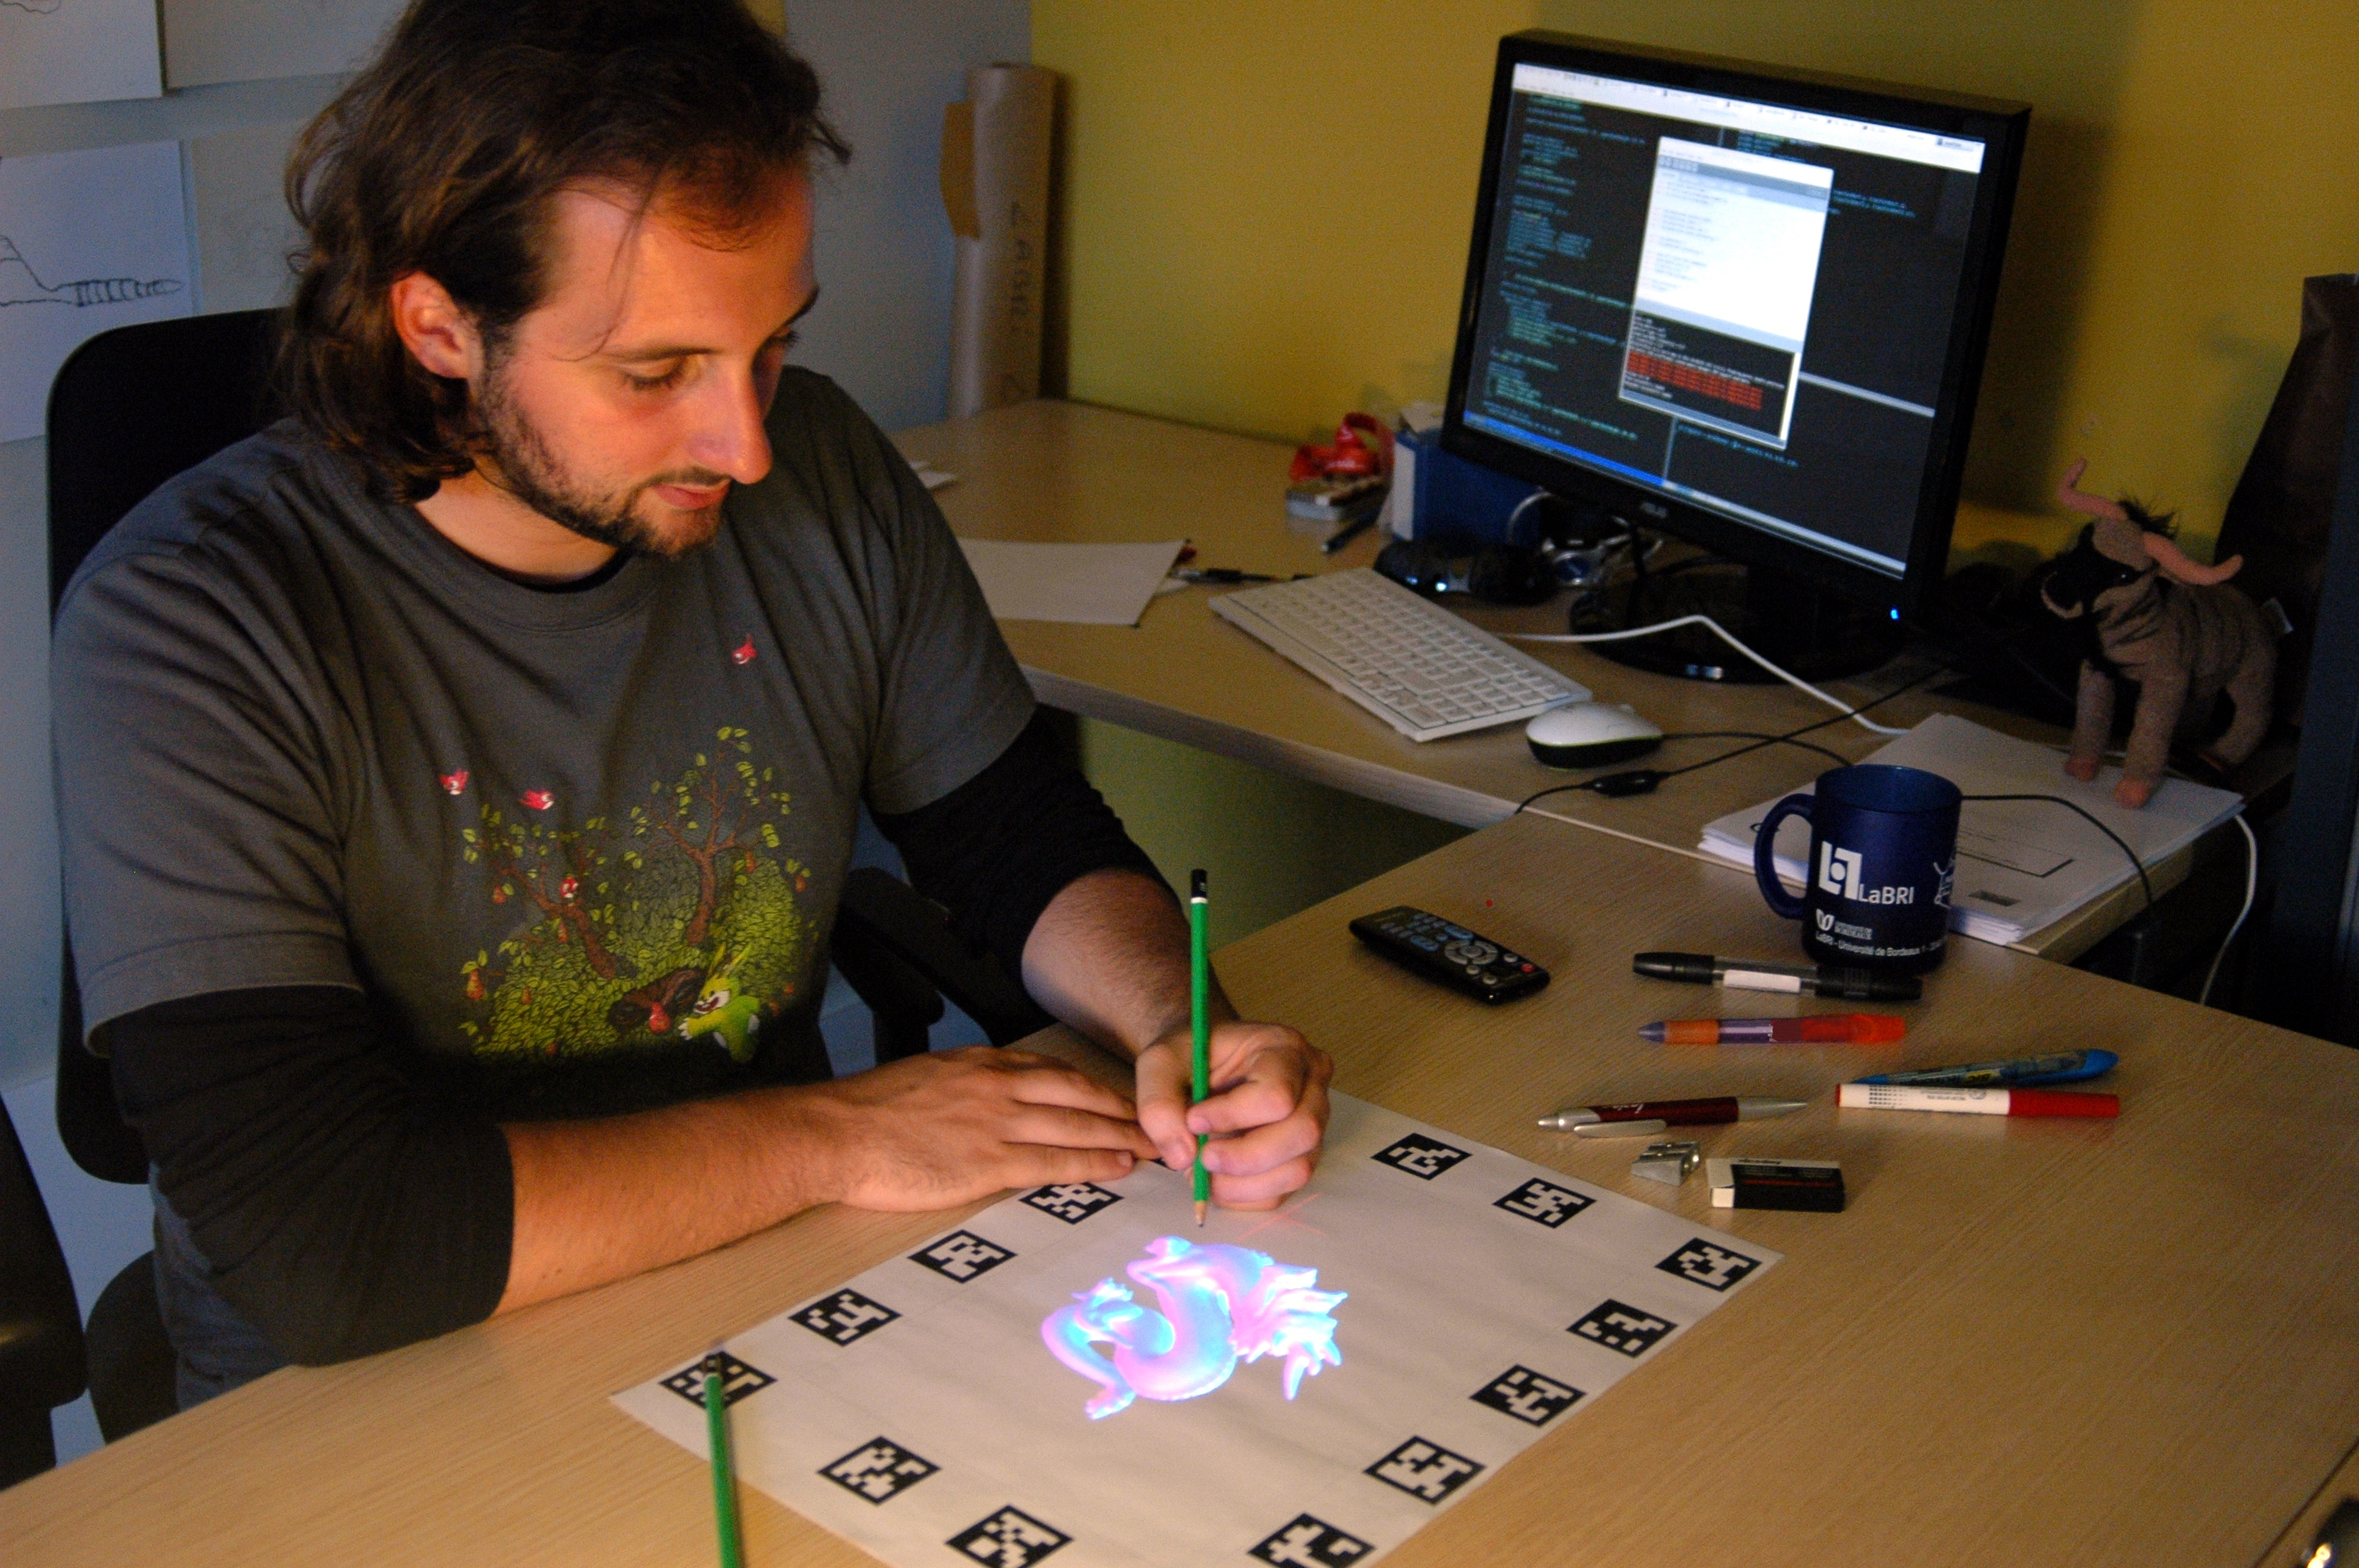
\includegraphics[width=0.65\textwidth]{images/papart-demo}
\caption{Jeremy Laviole utilisant PapARt pour dessiner en réalité augmentée\protect\footnotemark}
\label{fig:papartdemo}
\end{figure}
\footnotetext{Source: \href{https://team.inria.fr/potioc/fr/scientific-subjects_old/papart/}{Inria - PapARt}}

Le système interactif (fig~\ref{fig:papartsystem}) permettant d'utiliser tout le potentiel de PapARt est très spécifique. 

Il se compose de 2 dispositifs d'acquisitions, une caméra couleur observant la zone de travail pour venir y détecter les feuilles de papier qui serviront de base à la projection. Les feuilles de papier détectées par PapARt sont ornés de marqueurs ARToolKitPlus\footnote{\href{https://github.com/paroj/artoolkitplus}{https://github.com/paroj/artoolkitplus}}, est une bibliothèque de détection de marqueurs fiduciaires \footnote{Un marqueur fiduciaire est un objet placé dans le champ de vision le plus souvent de système d'imagerie qui apparait sur l'image produite et qui va servir de point de repère ou de référence.}. Ces marqueurs une fois détectés permettent d'estimer assez précisément la position de la feuille. Une fois la feuille détectée, PapARt se charge ensuite d'interpréter les marqueurs pour y projeter le contenu adéquat comme par exemple un dessin ou un menu.

Le deuxième dispositif d'acquisition est une caméra de profondeur qui a pour rôle de détecter les différents utilisateurs et les potentiels interactions. Grâce aux informations de profondeur, les interactions peuvent être détecté soit sur le plan de la zone de travail, ce sont des interactions qualifiées de "touch", soit dans l'espace au dessus de la zone de travail, qu'on qualifiera de "pointage 3D".
En plus de ces deux caméra, un projecteur est présent pour gérer toute la partie visualisation. Son rôle est de projeter dans les zones adéquates (i.e détectées via des feuilles de marqueur) le contenu numérique désiré. 

Pour avoir une représentation a l'échelle comme mentionné, il est nécessaire d'avoir un calibration caméras/projecteur très précise. Cette calibration très précise permet aux système complet d'avoir des capacités d'interaction et de manipulation (toucher, balayage, balayage a deux doigts) d'une tablette tactile.
% Rajouter image du touch et reformuler en disant que c'est très important dans papart d'avoir une echelle etc

\begin{figure}[H]
\centering
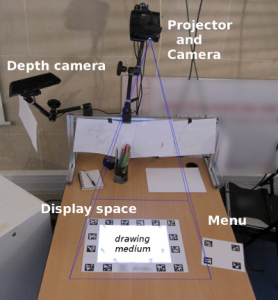
\includegraphics[width=0.4\textwidth]{images/papart-system}
\caption{Système interactif utilisant PapARt\protect\footnotemark}
\label{fig:papartsystem}
\end{figure}

\footnotetext{Source: \href{https://team.inria.fr/potioc/fr/scientific-subjects_old/papart/}{Inria - PapARt}}

Au delà des applications d'aide au dessins qui sont extrêmement nombreuses, PapARt ouvre un champ des possible assez large. Le rôle de RealityTech est d'explorer ce champ des possibles en améliorant PapARt et en fournissant de nouveau cas d'utilisation toujours plus innovants.

% Mettre des exemples


\section{Systèmes de réalité augmentée spatiale}
\label{sec:SARother}
\paragraph{RoomAliveToolKit} RoomAliveToolKit\cite{Jones:2014:RME:2642918.2647383} est un projet tout droit sorti des laboratoires de recherche de Microsoft. RoomAliveToolKit est un kit de développement créé en 2013 par Nikunj Raghuvanshi, Eyal Ofek et Andy Wilson qui permet, a l'instar de PapARt, de créer des expériences de projection interactive. La principale différence réside dans le fait que RoomAliveToolKit a pour but de donner vie à des pièces entière en utilisant plusieurs projecteurs et plus caméra qui fonctionne a l'unisson.

RoomAliveToolKit a permis entre autre de développer de nombreux projets basés sur de la projection interactive tel que RoomAlive, Room2Room, IllumiRoom et bien d'autre.

\begin{figure}[H]
    \centering
	\subfloat[Système de projection interactive nécessaire a l'utilisation de RoomAliveToolkit\protect\footnotemark]{
      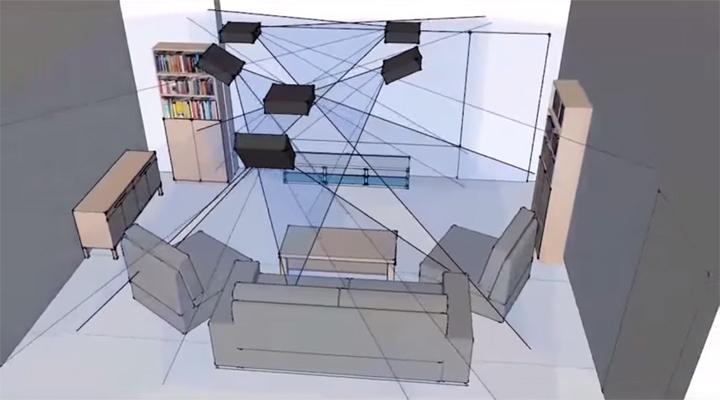
\includegraphics[width=0.45\textwidth]{images/roomalivesystem}
      \label{sub:roomalivesystem}
      }
    \subfloat[RoomAlive - Démonstration\protect\footnotemark]{
      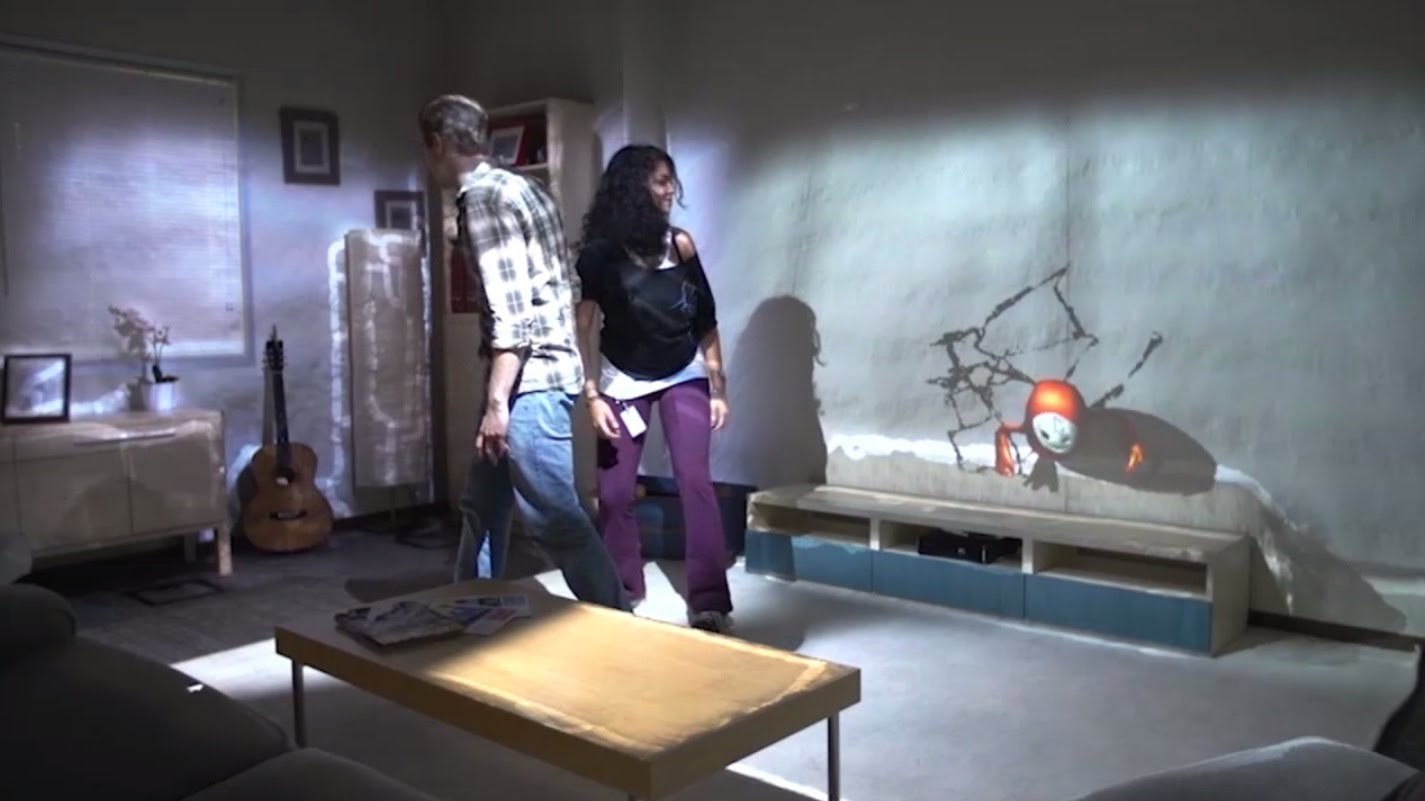
\includegraphics[width=0.45\textwidth]{images/roomalivedemo}
      \label{sub:roomalivedemo}
      }
\caption{Microsoft Research: RoomAliveToolkit et RoomAlive}
\label{fig:STAR}
\end{figure}
\footnotetext{Source: \href{https://pokemongolive.com/fr/}{RoomAliveToolkit}}
\footnotetext{Source: \href{https://www.microsoft.com/fr-fr/hololens}{Microsoft HoloLens}}


% Parler de la mise en place de la coordination de plusieurs projecteurs, des illusions projectives, 

\section{Bilan}